\documentclass[smaller]{beamer}
\usetheme[english]{Berlin}
\usepackage{ngerman}
\useoutertheme{infolines}
\beamertemplatenavigationsymbolsempty
\setbeamertemplate{caption}[numbered]
\usepackage{pgfplots,tikz,subfigure}
\usepackage{amsmath,amsthm}
\usepackage{hyperref,graphics,graphicx,color,algorithm,algorithmic,enumerate}
\usepackage{mymacros,wrapfig,relsize}
\usepackage{pict2e}
\usepackage[utf8x]{inputenc}

\newcommand{\ri}{\mathrm{i}}
\newcommand{\T}{\mathsf{T}}
\renewcommand{\H}{\mathsf{H}}
\newcommand{\eps}{\varepsilon}
\newcommand{\To}{\rightarrow}
\newcommand{\sddots}{\scalebox{0.6}{$\ddots$}}
\usepackage[pdf]{pstricks}
\usepackage{sansmathfonts}
\usepackage{eurosym}
\usepackage{ulem}
%\usepackage{arev}
%\renewcommand\familydefault{\sfdefault}

\DeclareMathOperator{\loc}{loc}
\DeclareMathOperator{\rank}{rank}
\DeclareMathOperator{\RE}{Re}
\DeclareMathOperator{\IM}{Im}
\DeclareMathOperator{\In}{In}
\DeclareMathOperator{\im}{im}
\DeclareMathOperator{\Gl}{Gl}
\DeclareMathOperator{\spa}{span}
\DeclareMathOperator{\ext}{{ext}}
\DeclareMathOperator{\ind}{ind}
\DeclareMathOperator{\normalrank}{normalrank}
\DeclareMathOperator{\essup}{ess\,sup}
\DeclareMathOperator{\vect}{vec}

\newcommand{\re}{\mathrm{e}}
\newcommand{\ddt}{\tfrac{\mathrm{d}}{\mathrm{d}t}}
\newcommand{\sys}[4]{\left[\begin{array}{c|c} #1 & #2 \\ \hline #3 & #4 \end{array}\right]}

\renewcommand{\tilde}{\widetilde}
\renewcommand{\hat}{\widehat}


\title[]{Optimierung f\"ur Studierende der Informatik}
\subtitle{-- 7. Vorlesung --}
\author[Matthias Voigt]{\textbf{Matthias Voigt$^{1,2}$}}
\institute[]{
\begin{columns}
%\begin{center}
\column{0.45\textwidth}{\centering {$^1$Universit\"at Hamburg \\ Fachbereich Mathematik \\ Hamburg \\ }}
\column{0.45\textwidth}{\centering {$^2$Technische Universit\"at Berlin \\ Institut f\"ur Mathematik \\ Berlin  \\}}
%\end{center}
\end{columns}
}
\date[]{Universit\"at Hamburg
\begin{columns}
\column{0.45\textwidth}{\centering 
\includegraphics[width = 1.2\textwidth]{uhh-logo.png}\\}
\end{columns}
}

\definecolor{tucgreen}{rgb}{0.0,0.5,0.27}
\definecolor{tucred}{rgb}{0.75,0,0}
\definecolor{tucorange}{rgb}{1.0,.5625,0}
\definecolor{mpired}{HTML}{990000}
\definecolor{mpigreen}{HTML}{5C871D}
\definecolor{mpiblue}{HTML}{006AA9}
\definecolor{mpibg1}{HTML}{5D8B8A}
\definecolor{mpibg2}{HTML}{BFDFDE}
\definecolor{mpibg3}{HTML}{A7C1C0}
\definecolor{mpibg4}{HTML}{7DA9A8}
\definecolor{mpigrey}{rgb}{0.9294,0.9294,0.8784}

\begin{document}

\maketitle

\begin{frame}
 \frametitle{Flussvergrößernde Pfade}
 Gegeben sei ein Netzwerk $N=(G,c,s,t)$ mit $G=(V,E)$ sowie ein Fluss $f$ auf $N$. \\ \vspace*{0.2cm}
 
 Existiert ein flussvergrößernder Pfad $P$, so kann man $P$ dazu benutzen, um aus $f$ einen Fluss $f^+$ zu gewinnen, \alert{für den $w(f^+) > w(f)$ gilt.} \\ \vspace*{0.2cm}
 
 Anhand unseres Beispiels hatten wir dies bereits gesehen -- allgemein geht dies wie folgt:
\end{frame}

\begin{frame}
 \frametitle{Definition von $d$}
 Zu jeder Kante von $P$ definieren wir eine Zahl $d_i$, indem wir \alert{für Vorwärtskanten} $(v_i, v_{i+1})$ festsetzen:
\[
d_i = c(v_i,v_{i+1}) - f(v_i,v_{i+1});
\]

\alert{für Rückwärtskanten} sei dagegen
\[
d_i = f(v_{i+1},v_i).
\]

Dann gilt in jedem Fall $d_i > 0$. Wir setzen
\[
d := \min \big\{ d_i \; : \; i = 1,\ldots,k-1 \big\},
\]
d.h., $d$ ist der kleinste Wert unter den $d_i$. Es gilt $d > 0$.
\end{frame}

\begin{frame}
\frametitle{Definition des neuen Flusses}
\alert{Wir definieren den neuen Fluss $f^+$ wie folgt:}
\begin{itemize}
\item Es gelte $f^+(v_i, v_{i+1}) = f(v_i, v_{i+1}) + d$, falls $(v_i, v_{i+1})$ eine Vorwärtskante von $P$ ist.
\item Falls $(v_{i+1},v_i)$ eine Rückwärtskante von $P$ ist, so sei $f^+(v_{i+1},v_i) = f(v_{i+1},v_i)-d$.
\item Für alle anderen Kanten $e$ lassen wir den Fluss durch $e$ unverändert, d.h. $f^+(e)=f(e)$.
\end{itemize}
\vspace*{0.2cm}
Aufgrund der Konstruktion von $f^+$ gilt dann: $f^+$ ist ein Fluss auf $N$ mit
\begin{equation}
\label{eq:9:9}
w(f^+) = w(f) + d.
\end{equation}

Wegen $d > 0$ haben wir also $w(f^+) > w(f)$.
\end{frame}

\begin{frame}
 \frametitle{Ganzzahlige Flüsse}
 \textbf{Man beachte:} Alle Kapazitäten sind ganze Zahlen, da wir ja $c(e) \in \N \cup \bigl\{ 0 \bigr\}$ für alle Kanten $e \in E$ voraussetzen. \\ \vspace*{0.2cm}

Sind auch alle $f(e)$ ganze Zahlen, so sprechen wir von einem \structure{ganzzahligen Fluss}. \\ \vspace*{0.2cm}

Ist $f$ ein ganzzahliger Fluss, so folgt aus der Definition von $d$, dass auch $d$ eine ganze Zahl ist und dass somit $d \geq 1$ gilt. Wir halten fest:
\begin{equation}
\label{eq:9:10}
\alert{\text{Ist $f$ ganzzahlig, so auch $f^+$, und es gilt $w(f^+) \geq w(f)+1$.}}
\end{equation}

Unsere Überlegungen legen das folgende \alert{Verfahren zur Bestimmung eines maximalen Flusses} in einem Netzwerk nahe.
\end{frame}

\begin{frame}
 \frametitle{Die Ford-Fulkerson-Methode}
 \textbf{Algorithmus:} Ford-Fulkerson-Methode
\begin{enumerate}[\bfseries 1.]
\item Man startet mit dem \alert{Nullfluss} $f_0$: Dies ist der (ganzzahlige) Fluss, für den $f_0(e) = 0$ für alle $e \in E$ gilt.
\item Ist bereits ein ganzzahliger Fluss $f_n$ konstruiert, so suche man nach einem $f_n$-vergrößernden Pfad $P$. Es ist nicht schwer, diese Suche systematisch zu betreiben; {Details hierzu werden später besprochen.}
\begin{enumerate}[\bfseries 1.]
\item Existiert ein solches $P$, so benutze man $P$, um aus $f_n$ einen ganzzahligen Fluss $f_{n+1}$ mit $w(f_{n+1}) \geq w(f_n)+1$ zu gewinnen; man wiederhole dann 2. mit $f_{n+1}$ anstelle von $f_n$.
\item Existiert kein solcher Pfad $P$, so ist man fertig, da -- wie wir gleich sehen werden -- in diesem Fall ein Schnitt $(S,T)$ mit $w(f_n) = c(S,T)$ existiert, was ja bedeutet, dass $w(f_n)$ maximal sein muss.
\end{enumerate}
\end{enumerate}
\end{frame}

\begin{frame}
 \frametitle{Die Ford-Fulkerson-Methode}
 Der \textbf{wichtigste Punkt}, der noch zu klären ist, betrifft die in \textbf{2.2.} gemachte Aussage, dass es im Fall, dass kein $f_n$-vergrößernder Pfad existiert, immer einen Schnitt $(S,T)$ mit
\begin{equation}
\label{eq:9:11}
w(f_n) = c(S,T)
\end{equation}
geben muss. \\ \vspace*{0.2cm}

Wir werden sehen, dass man als Ergebnis des Ford-Fulkerson-Algorithmus nicht nur einen Maximalfluss $f_n$ erhält, sondern \alert{dass man im letzten Schritt des Verfahrens gleichzeitig auch einen Schnitt $(S,T)$, für den \eqref{eq:9:11} gilt, ganz umsonst mitgeliefert bekommt}.
\end{frame}

\begin{frame}
 \frametitle{Zertifikat für die Optimalität}
 Am Ende des Verfahrens erhält man also neben einem maximalen Fluss auch einen minimalen Schnitt \alert{und hat somit ein \textbf{Zertifikat für die Optimalität des gefundenen Flusses} in der Hand}: \\ \vspace*{0.2cm}
 
 Stellen Sie sich vor, dass jemand anderes bezweifelt, dass der von Ihnen gefundene Fluss $f^*$ tatsächlich maximal ist. Dann brauchen Sie nur den ebenfalls gefundenen minimalen Schnitt $(S^*,T^*)$ aus der Tasche zu holen und darauf hinzuweisen, dass
\[ 
w(f^*) = c(S^*,T^*)
\]
gilt: Ihr Gegenüber wird sofort verstummen. \\ \vspace*{0.2cm}

Beim Ford-Fulkerson-Verfahren handelt es sich also (ebenso wie beim Simplexverfahren) um einen \alert{zertifizierenden Algorithmus}.
\end{frame}

\begin{frame}
 \frametitle{Der noch fehlende Baustein}
 \textbf{Feststellung 3:} Ist $N = (G,c,s,t)$ ein Netzwerk mit $G=(V,E)$ und ist $f$ ein Fluss auf $N$, für den es keinen $f$-vergrößernden Pfad $P$ gibt, so existiert ein Schnitt $(S,T)$ mit $$w(f) = c(S,T).$$ \\ \vspace*{0.2cm}

Bevor wir diese Feststellung beweisen, erläutern wir die \alert{Grundidee}: Stellen Sie sich vor, dass Sie in der $n$-ten Iteration des Ford-Fulkerson-Verfahrens den Fluss $f_n$ erhalten haben und dass $f_n$ maximal ist -- was Sie allerdings noch nicht wissen. Sie steigen also in die $(n+1)$-te Iteration ein und versuchen einen $f_n$-vergrößernden Pfad $P$ zu konstruieren, wobei Sie bei der Quelle $s$ starten und versuchen, die Senke $t$ mit einem solchen Pfad zu erreichen. 
\end{frame}

\begin{frame}
 \frametitle{Grundidee des Beweises von Feststellung 3}
 Da $f_n$ bereits maximal ist, wird das nicht gelingen -- Sie werden immer nur Knoten $v \neq t$ erreichen. \\ \vspace*{0.2cm}
 
  Die Menge aller Knoten $v$, die Sie auf diese Art erreichen können, nennen wir $S$; die Menge der übrigen Knoten nennen wir $T$. \\ \vspace*{0.2cm}

 Es ist nicht schwer, sich zu überlegen, dass für den auf diese Art gefundenen Schnitt $(S,T)$ gilt: $$w(f_n) = c(S,T);$$ dass dies tatsächlich so ist, wird im Folgenden nachgewiesen.
\end{frame}

\begin{frame}
 \frametitle{Definition von $(S,T)$}
  \textbf{Beweis von Feststellung 3:} Wir definieren $S$ als die Menge derjenigen $v \in V$, für die es einen zunehmenden Pfad nach $v$ gibt. \\ \vspace*{0.2cm}

  Dann gilt $s \in S$, da der einpunktige Pfad, der nur aus $s$ besteht, ein zunehmender Pfad nach $s$ ist. \\ \vspace*{0.2cm} 
  
  Außerdem gilt $t \not\in S$, da es andernfalls einen $f$-vergrößernden Pfad geben würde. \\ \vspace*{0.2cm}
  
  Wir setzen $T = \overline{S}$. Es handelt sich bei $(S,T)$ also um einen Schnitt. \alert{Wir zeigen nun, dass für diesen Schnitt $(S,T)$ gilt:}
 \begin{equation} \label{eq:9:12}
 w(f) = c(S,T).
 \end{equation}
\end{frame}

\begin{frame}
 \frametitle{Nachweis von \eqref{eq:9:12}}
 Zum Nachweis von \eqref{eq:9:12} sei $(x,y)$ eine beliebige Kante aus $E$ mit $x \in S$ und $y \in T$. \\ \vspace*{0.2cm}
 
 Wegen $x \in S$ existiert ein zunehmender Pfad nach $x$, den wir $P_x$ nennen wollen (siehe Zeichnung). 
 
 \begin{center}
  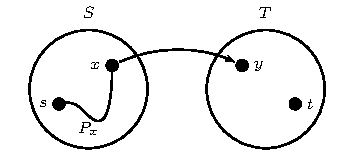
\includegraphics{fig19.pdf}
 \end{center}
Es folgt $f(x,y) = c(x,y)$, \alert{da man andernfalls $P_x$ zu einem zunehmenden Pfad nach $y$ verlängern könnte}, im Widerspruch zu $y \not\in S$.
\end{frame}

\begin{frame}
 \frametitle{Nachweis von \eqref{eq:9:12}}
 Da $(x,y)$ eine beliebige Kante aus $E$ mit $x \in S$ und $y \in T$ ist, gilt also $f(x,y) = c(x,y)$ für alle derartigen Kanten, d.h., es gilt:
\[
f^+(S) = f(S,T) = c(S,T).
\]

Auf eine ganz ähnliche Art findet man, dass gilt (Übungsaufgabe!):
\[
f^-(S) = f(T,S) = 0.
\]

Aufgrund des Hilfssatzes (siehe Vorlesung 6) wissen wir, dass
\[
w(f) = f^+(S) - f^-(S)
\]
gilt. Insgesamt ergibt sich demnach:
\[
w(f) = f^+(S) - f^-(S) = c(S,T). \qquad \Box
\]
\end{frame}

\begin{frame}
 \frametitle{Terminierung}
 Ist $K = \sum\limits_{e \in E}{c(e)}$ die Summe aller in $N$ vorkommenden Kantenkapazitäten, so gilt aufgrund von Feststellung 2 natürlich $w(f) \leq K$. \\ \vspace*{0.2cm}
 
 \alert{Dadurch ist sichergestellt, dass man beim Ford-Fulkerson-Verfahren nach endlich vielen Flussvergrößerungen fertig ist. (Man beachte vor allem (\ref{eq:9:10})!)} \\ \vspace*{0.2cm}

Das Verfahren terminiert also, man kommt nach endlich vielen Flussvergrößerungen zu \textbf{2.2.}, womit auch das \alert{Max-Flow Min-Cut Theorem} bewiesen ist.
\end{frame}

\begin{frame}
 \frametitle{Labelling-Algorithmus}
 Das Ford-Fulkerson-Verfahren wird in der englischsprachigen Literatur auch
\begin{center}
\structure{labelling algorithm}
\end{center}
genannt; wir werden in Kürze sehen, woher der Name kommt. \\ \vspace*{0.2cm}

Auf Deutsch sagt man übrigens \structure{Labelling-Algorithmus} oder \structure{Markierungsalgorithmus}. \\ \vspace*{0.2cm}

In diesem Abschnitt sind wir (zumindest teilweise) der Darstellung in den folgenden Büchern gefolgt:
\begin{itemize}
\item D. Jungnickel: \textit{Graphs, Networks and Algorithms}. Springer-Verlag. 2012. 4. Auflage.
\item A. Beutelspacher, M.-A. Zschiegner: \textit{Diskrete Mathematik für Einsteiger}. Vieweg-Verlag. 2014. 5. Auflage.
\end{itemize}
\end{frame}

\begin{frame}
 \frametitle{Weitere Deatils des Labelling-Algorithmus}
 \alert{Wir besprechen nun weitere Details des Labelling-Algorithmus}, wobei wir verstärkt nach Jungnickel vorgehen; unter anderem lernen wir auch den \structure{Algorithmus von Edmonds und Karp} kennen. \\ \vspace*{0.2cm}

Eine Bezeichnung, die im Jungnickel häufig auftaucht: Ist $e$ eine Kante eines Digraphen, so bezeichnet \alert{$e^-$ den Anfangsknoten} und \alert{$e^+$ den Endknoten von $e$}.
\begin{center}
 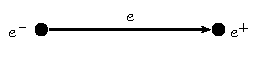
\includegraphics{fig20.pdf}
\end{center}

\end{frame}

\begin{frame}
 \frametitle{Labelling-Algorithmus (Grobform)}
   Hier zunächst einmal der \alert{Labelling-Algorithmus in Grobform}, wie er im Jungnickel beschrieben wird\footnote{Um einen flussvergrößernden Pfad $P$ zu beschreiben, genügt es, die Kanten von $P$ anzugeben. In (3) wird deshalb $P=(e_1,\ldots,e_r)$ geschrieben.}:
 %  \begin{center}
\begin{tabular}{rl}
(1)& $f(e) \leftarrow 0$ für alle Kanten $e$; \\
(2)& \textbf{while} $\exists$ $f$-vergrößernder Pfad \textbf{do} \\
(3)& \qquad Sei $P = (e_1,\ldots,e_r)$ ein $f$-vergrößernder Pfad von $s$ nach $t$. \\
(4)& \qquad $d \leftarrow \min \bigl( \bigl\{ c(e_i)-f(e_i) : e_i$ ist eine Vorwärtskante von $P \bigr\}$ \\
   & \qquad\qquad\qquad\quad $\cup\ \bigl\{ f(e_i) : e_i$ ist eine Rückwärtskante in $P \bigr\} \bigr)$. \\
(5)& \qquad $f(e_i) \leftarrow f(e_i) + d$ für jede Vorwärtskante $e_i$. \\
(6)& \qquad $f(e_i) \leftarrow f(e_i) - d$ für jede Rückwärtskante $e_i$. \\
(7)& \textbf{end do}
\end{tabular}
%\end{center}
\end{frame}

\begin{frame}
 \frametitle{Markierungen}
 Die Markierungen (labels) sind in dieser Grobform noch nicht vorhanden. Sie kommen erst ins Spiel, wenn es um die \alert{Details} geht:
 \begin{itemize}
  \item Es ist noch festzulegen, auf welche Art die Suche nach einem flussvergrößernden Pfad erfolgen soll.
  \item Es bietet sich an, die Suche nach einem solchen Pfad und die Berechnung von $d$ geeignet zu kombinieren. 
  \item Und schließlich wollen wir ja gar nicht nur einen maximalen Fluss, sondern auch einen minimalen Schnitt bestimmen. 
 \end{itemize}
 \alert{All dies führt zur Verwendung von {\glqq}labels{\grqq}.} Es sind übrigens die Knoten, die markiert werden; es geht also nicht um Kanten-, sondern um \alert{Knotenmarkierungen}.
\end{frame}

\begin{frame}
 \frametitle{Labelling-Algorithmus}
  %Hier nun die Details des Labelling-Algorithmus (aus Jungnickel: \textit{Graphs, Networks and Algorithms}, Springer-Verlag (2012, 4. Auflage)): \\ \vspace*{0.2cm}

\begin{tabular}{rl}
%\multicolumn{2}{l}{\textbf{Labelling algorithm of Ford and Fulkerson}.} \\
%\multicolumn{2}{l}{Let $N = (G, c, s, t)$ be a flow network.} \\
%& \\
%\multicolumn{2}{l}{\textbf{Procedure} FORDFULK$(N, f, S, T)$} \\
 (1)& \textbf{for} $e \in E$ \textbf{do} $f(e) \leftarrow 0$ \textbf{end do} \\
 (2)& Markiere $s$ mit $(\star,\star,\infty)$. \\
 (3)& \textbf{for} $v \in V$ \textbf{do} $u(v) \leftarrow$ false; $d(v) \leftarrow \infty$ \textbf{end do} \\
 (4)& \textbf{repeat} \\
 (5)& \qquad Wähle einen markierten Knoten $v$, der $u(v) =$ false erfüllt. \\
 (6)& \qquad \textbf{for} $e \in \big\{ e \in E : e^- = v \big\}$ \textbf{do} \\
 (7)& \qquad\qquad \textbf{if} $w=e^+$ ist nicht markiert und $f(e) < c(e)$ \textbf{then} \\
 (8)& \qquad\qquad\qquad $d(w) \leftarrow \min \big\{ c(e)-f(e), d(v) \big\}$. \\
 (9)& \qquad\qquad\qquad Markiere $w$ mit $(v,+, d(w))$. \\
 (10)& \qquad\qquad \textbf{end if} \\
 (11)& \qquad \textbf{end do} \\
 (12)& \qquad \textbf{for} $e \in \bigl\{ e \in E : e^+ = v \bigr\}$ \textbf{do} \\
 (13)& \qquad\qquad \textbf{if} $w=e^-$ is nicht markiert and $f(e)>0$ \textbf{then} \\
 (14)& \qquad\qquad\qquad $d(w) \leftarrow \min \big\{ f(e), d(v) \big\}$. \\
 (15)& \qquad\qquad\qquad Markiere $w$ mit $(v,-, d(w))$. \\
 (16)& \qquad\qquad \textbf{end if} \\
 (17)& \qquad \textbf{end do} \\
\end{tabular}
\end{frame}

\begin{frame}
\frametitle{Labelling-Algorithmus}
\begin{tabular}{rl}
(18)& \qquad $u(v) \leftarrow$ true; \\
(19)& \qquad \textbf{if} $t$ ist markiert \textbf{then} \\
(20)& \qquad\qquad Sei $d$ die letzte Komponente der Markierung von $t$. \\
(21)& \qquad\qquad $w \leftarrow t$. \\
(22)& \qquad\qquad \textbf{while} $w \neq s$ \textbf{do} \\
(23)& \qquad\qquad\qquad Bestimme die erste Komponente $v$ der Markierung von $w$. \\
(24)& \qquad\qquad\qquad \textbf{if} die zweite Komponente der Markierung von $w$ ist $+$ \textbf{then} \\
(25)& \qquad\qquad\qquad\qquad Setze $f(e) \leftarrow f(e) + d$ für $e=(v,w)$. \\
(26)& \qquad\qquad\qquad \textbf{else} \\
(27)& \qquad\qquad\qquad\qquad Setze $f(e) \leftarrow f(e) - d$ für $e=(w,v)$. \\
(28)& \qquad\qquad\qquad \textbf{end if} \\
(29)& \qquad\qquad\qquad $w \leftarrow v$. \\
(30)& \qquad\qquad \textbf{end do} \\
(31)& \qquad\qquad Lösche alle Markierungen außer der Markierung von $s$. \\
(32)& \qquad\qquad \textbf{for} $v \in V$ \textbf{do} $d(v) \leftarrow \infty$; $u(v) \leftarrow$ false \textbf{end do} \\
(33)& \qquad \textbf{end if} \\
(34)& \textbf{until} $u(v) =$ true für alle markierten Knoten $v$. \\
(35)& Sei $S$ die Menge aller markierten Knoten und setze $T \leftarrow V \setminus S$.
\end{tabular}
\end{frame}

\begin{frame}
 \frametitle{Der Algorithmus von Edmonds und Karp}
 Einen \alert{Schönheitsfehler} hat der vorgestellte Algorithmus allerdings noch. Das wird deutlich, wenn wir uns das folgende Beispiel anschauen:
 \begin{center}
  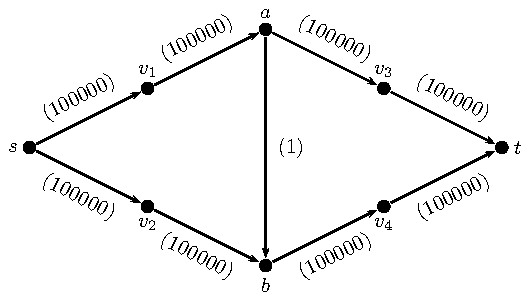
\includegraphics{fig21.pdf}
 \end{center}

\end{frame}

\begin{frame}
 \frametitle{200000 Iterationen bei 8 Knoten}
 Die geklammerten Zahlen an den Kanten sind die Kapazitäten. Man sieht sofort, dass der \alert{optimale Flusswert gleich 200000} ist. \\ \vspace*{0.2cm}

Wendet man das Ford-Fulkerson-Verfahren an, so könnte es einem bei ungeschickter Wahl der flussvergrößernden Pfade passieren, dass in jeder Iteration der Fluss nur um den Wert 1 wächst. (Wie nämlich?) \\ \vspace*{0.2cm}

\alert{Man wäre also erst nach 200000 Iterationen fertig} -- und das, obwohl das Netzwerk nur 8 Knoten hat! \\ \vspace*{0.2cm}

Dieses Defizit des Labelling-Algorithmus gilt es zu beseitigen. Der folgende Satz von Edmonds und Karp zeigt, wie das geschehen kann. Der Beweis des Satzes von Edmonds und Karp ist nicht schwierig. %Am Ende dieses Abschnitts wird ein Beweis vorgestellt.
\end{frame}

\begin{frame}
 \frametitle{Der Satz von Edmonds und Karp}
 \textbf{Satz (Edmonds und Karp, 1972):}
Wählt man im Labelling-Algorithmus den flussvergrößernden Pfad $P$ immer so, dass $P$ \alert{möglichst wenige Kanten} enthält, so terminiert der Algorithmus nach höchstens
\[
\left\lfloor \frac{(n-1)m}{2} \right\rfloor
\]
Flussvergrößerungen (für $n = |V|$ und $m = |E|$). 
\end{frame}

\begin{frame}
 \frametitle{Edmonds/Karp liefert eine von den Kapazitäten unabhängige Schranke}
 Im Satz von Edmonds und Karp wird also eine obere Schranke für die Zahl der Flussvergrößerungen angegeben, die \alert{unabhängig von der Größe der Kapazitäten} ist. Stattdessen ist die angegebene Schranke nur von der Knotenzahl $n=|V|$ und der Kantenzahl $m=|E|$ abhängig. \\ \vspace*{0.2cm}
 
 \alert{Allerdings muss sichergestellt sein, dass auch immer ein möglichst kurzer flussvergrößernder Pfad ausgewählt wird}, wobei {\glqq}möglichst kurz{\grqq} natürlich bedeuten soll, dass $P$ unter allen flussvergrößernden Pfaden möglichst wenige Kanten besitzt. \\ \vspace*{0.2cm}

\alert{Dies ist nicht schwer zu erreichen}, man erledigt dies, indem man in Zeile (5) des Algorithmus wie bei einer \structure{Breitensuche} vorgeht.
\end{frame}

\begin{frame}
 \frametitle{Der Algorithmus von Edmonds und Karp}
 Hierzu ist (5) nur durch die modifizierte Zeile (5') zu ersetzen: \\ \vspace*{0.2cm}

\begin{tabular}{rl}
(5')& Unter allen Knoten mit $u(v) =$ false, sei $v$ der Knoten,  \\
    & der zuerst markiert wurde.
\end{tabular}
\label{page:9:6}
\vspace*{0.2cm}

Der Unterschied zwischen (5) und (5') liegt auf der Hand:
\begin{itemize}
\item In (5) wird ein Knoten $v$, der markiert ist, aber noch nicht inspiziert wurde, \alert{beliebig} ausgewählt.
\item Dagegen wird in (5') unter allen Knoten, die markiert sind, aber noch nicht inspiziert wurden, derjenige Knoten $v$ ausgewählt, \alert{der zuerst markiert wurde}.
\end{itemize}
\end{frame}

\begin{frame}
 \frametitle{First Labelled -- First Scanned}
 Den derart modifizierten Labelling-Algorithmus ({\glqq}Ersetzung von (5) durch (5'){\grqq}) nennt man den \structure{Algorithmus von Edmonds und Karp}. Das Neue am Algorithmus von Edmonds und Karp ist, dass in (5') nach dem folgenden Motto vorgegangen wird: \\ \vspace*{0.2cm}

\begin{center}
\alert{first labelled -- first scanned.}
\end{center}
\vspace*{0.2cm}
Umsetzen lässt sich (5') dadurch, dass man die markierten, aber noch nicht inspizierten Knoten mithilfe einer \alert{Warteschlange} verwaltet. \\ \vspace*{0.2cm}

\end{frame}

\begin{frame}
 \frametitle{Ein Beispiel}
 %Das nachfolgende, etwas umfangreichere Beispiel illustriert die Arbeitsweise des Algorithmus von Edmonds und Karp. \\ \vspace*{0.2cm}

\textbf{Beispiel} (aus Jungnickel): Es geht um das folgende Netzwerk $N$, bei dem die Kapazitäten in Klammern angegeben sind:
 \begin{center}
 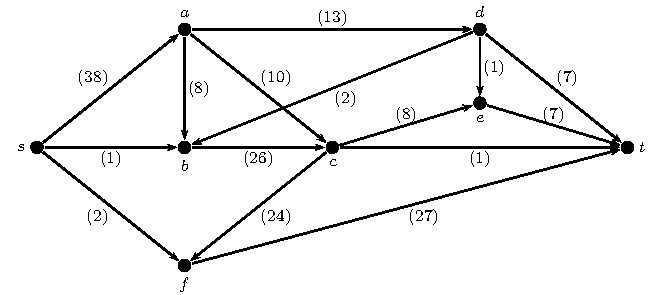
\includegraphics{fig22.pdf}
\end{center}
Wir bestimmen nun für $N$ einen maximalen Fluss und einen minimalen Schnitt. Die Zahlen ohne Klammern geben den Fluss durch die einzelnen Kanten an, wobei es natürlich mit dem Nullfluss losgeht.
\end{frame}

\begin{frame}
 \frametitle{Ein Beispiel}
 \begin{center}
  \begin{figure}
   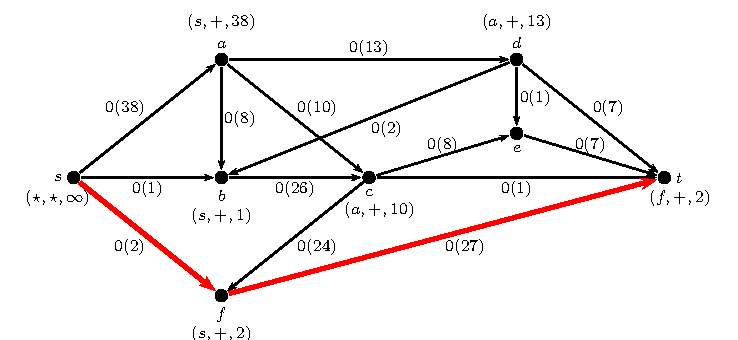
\includegraphics[scale=0.8]{fig23.pdf}
   \caption{$w(f_0) = 0$}
   \label{abb:9:2}
  \end{figure}
 \end{center}

 Die Knoten werden in Abbildung \ref{abb:9:2} in der Reihenfolge $s$, $a$, $b$, $f$, $c$, $d$, $t$ markiert; $e$ wird nicht markiert, da bereits zuvor in Zeile (15) des Labelling-Algorithmus festgestellt wurde, dass die Senke $t$ mit einem Label versehen worden ist. Der gefundene flussvergrößernde Pfad wird immer \textcolor{red}{\textbf{fett}} gezeichnet.
\end{frame}

\begin{frame}
 \frametitle{Eine Zusatzregel}
  Wir beschreiben im Folgenden, wie die zuvor angegebene Reihenfolge der Knotenmarkierungen in Abbildung \ref{abb:9:2} zustande kommt. \\ \vspace*{0.2cm}
  
  Diese Reihenfolge ist nur zum Teil durch den Algorithmus von Edmonds und Karp vorgegeben; um eine vollständig festgelegte Reihenfolge zu erhalten, fügen wir die folgende \textbf{Regel} hinzu: \\ \vspace*{0.2cm}
%\begin{center}

\begin{tabular}{rl}
($*$)& Ist im Algorithmus von Edmonds und Karp die Reihenfolge der zu \\
         & markierenden Knoten nicht festgelegt, so soll die \alert{alphabetische Reihenfolge} \\
         & den Ausschlag geben.
\end{tabular}
%\end{center}
\label{page:9:8}
\\ \vspace*{0.2cm}
Wie wir wissen, geht es mit dem Nullfluss los (siehe Zeile (1) des Labelling-Algorithmus sowie Abbildung~\ref{abb:9:2}); anschließend erhält $s$ in Zeile (2) die Markierung $(\star,\star,\infty)$.
\end{frame}

\begin{frame}
\frametitle{Die Warteschlange $Q$}
Die Warteschlange, die die markierten, aber noch nicht inspizierten Knoten enthält, wollen wir mit $Q$ bezeichnen. Anfangs enthält $Q$ also nur den Knoten $s$, d.h., nach abgeschlossener Initialisierung (Zeile (1)--(3)) bietet sich für $Q$ das folgende Bild: 
\[
 Q:\ s.
\]

Beim ersten Durchlauf der in Zeile (4) beginnenden Repeat-Schleife wird in (5') als Knoten $v$ die Quelle $s$ gewählt; kurz: $v=s$. Danach erhalten die Knoten $a$, $b$ und $f$ ihre jeweiligen Markierungen (siehe Zeile (6)--(11) bzw. Abbildung \ref{abb:9:2}). Wegen ($*$) erfolgt dies in der alphabetischen Reihenfolge: Zuerst wird $a$ markiert, dann $b$ und danach $f$.
\end{frame}

\begin{frame}
 \frametitle{Erster Durchlauf der Repeat-Schleife}
 Die Ausführung der anschließenden Zeilen (12)--(17) entfällt, da es keine Kanten gibt, die in $s$ hineinführen. Damit sieht unsere Warteschlange $Q$ nun wie folgt aus:
\[
Q:\ s\ a\ b\ f.
\]

Da die Inspizierung von $s$ in Zeile (17) zum Abschluss gekommen ist, wird in Zeile (18) $u(s) = \text{true}$ gesetzt. Für die Warteschlange bedeutet dies, dass $s$ aus $Q$ gelöscht wird; wir stellen den Vorgang wie folgt dar:
\[
Q:\ \xout{s}\ a\ b\ f.
\]

In Zeile (19) wird gefragt, ob $t$ bereits markiert ist; da dies zu verneinen ist, entfällt die Ausführung der Zeilen (20)--(32). In Zeile (34) wird geklärt, ob die Repeat-Schleife noch ein weiteres Mal zu durchlaufen ist: Da es markierte, aber nicht inspizierte Knoten gibt ($Q$ ist nicht leer!), steigen wir bei (4) wieder ein.
\end{frame}

\begin{frame}
\frametitle{Weiterer Durchlauf der Repeat-Schleife}
\alert{Nun wirkt sich zum ersten Mal die Tatsache aus, dass (5) durch (5') ersetzt wurde:} In $Q$ steht $a$ an erster Stelle, d.h., in (5') setzen wir $v=a$. \\ \vspace*{0.2cm}

Anschließend wird (6)--(11) ausgeführt, was dazu führt, dass $c$ und $d$ ihre jeweiligen Markierungen bekommen (in dieser Reihenfolge); $b$ ist nicht zu berücksichtigen, da der Knoten $b$ bereits markiert ist. Bei der anschließenden Ausführung von (12)--(17) passiert nichts Erwähnenswertes: $(s,a)$ ist die einzige Kante, die in $a$ hineinführt -- und $s$ ist bereits markiert! Nach Ausführung von (18) gilt $u(a) = \text{true}$; für unsere Warteschlange bedeutet dies, dass sich $Q$ aktuell im folgenden Zustand befindet:
\[
Q:\ \xout{s}\ \xout{a}\ b\ f\ c\ d.
\]
\end{frame}

\begin{frame}
\frametitle{Weiterer Verlauf der 1. Iteration}
Nun wird wie zuvor fortgefahren: In (19) wird festgestellt, dass $t$ noch nicht markiert ist, weshalb es bei (34) weitergeht. Wegen $Q \neq \emptyset$ wird die Repeat-Schleife ein weiteres Mal durchlaufen, diesmal für $v=b$. Dies führt zu keinen weiteren Markierungen, da $a$, $c$, $d$ und $s$ bereits markiert sind; es wird $u(b) = \text{true}$ gesetzt und man erhält
\[
Q:\ \xout{s}\ \xout{a}\ \xout{b}\ f\ c\ d.
\]

Im nächsten Durchlauf der repeat-Schleife gilt $v=f$; zusätzlich markiert wird nur der Knoten $t$. Es wird $u(f) = \text{true}$ gesetzt, was zu
\[
Q:\ \xout{s}\ \xout{a}\ \xout{b}\ \xout{f}\ c\ d\ t
\]
führt. Bei der Abfrage in (19), ob $t$ markiert ist, lautet \alert{die Antwort diesmal ja.} Folglich werden diesmal die Zeilen (20)--(32) ausgeführt, was zu folgendem Resultat führt: 
\end{frame}

\begin{frame}
 \frametitle{Ende der 1. Iteration}
 Man erhält den flussvergrößernden Pfad $s,f,t$ (siehe Abbildung \ref{abb:9:2}) und der Fluss wird in den Kanten dieses Pfades um 2 erhöht (siehe Abbildung \ref{abb:9:3}). Die bisherigen Markierungen werden bis auf die Markierung von $s$ gelöscht und es wird $u(v)$ für alle Knoten $v$ auf false gesetzt. Für $Q$ bedeutet dies, dass $Q$ wie am Anfang nur noch $s$ enthält:
\[
Q:\ s.
\]

Da anschließend in (34) festgestellt wird, dass es markierte, aber nicht inspizierte Knoten gibt (Es gilt $Q \neq \emptyset$!), \alert{geht es in den nächsten Durchlauf der Repeat-Schleife, wobei $v=s$ gilt.} Hier nun der weitere Verlauf:
\end{frame}

\begin{frame}
 \frametitle{Weiterer Verlauf}
 \begin{center}
  \begin{figure}
   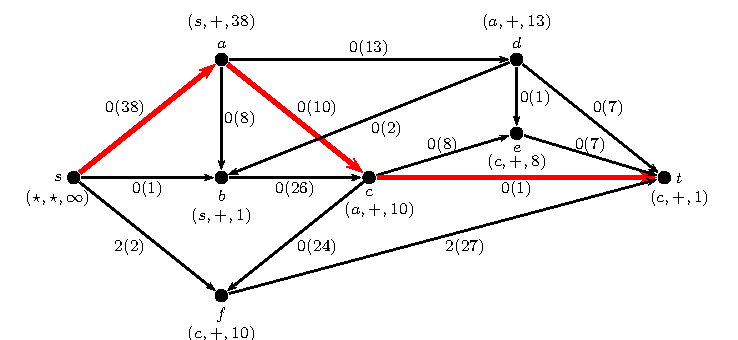
\includegraphics{fig24.pdf}
   \caption{$w(f_1) = 2$}
   \label{abb:9:3}
  \end{figure}
\end{center}
\end{frame}

\begin{frame}
 \frametitle{Weiterer Verlauf}
 \begin{center}
  \begin{figure}
   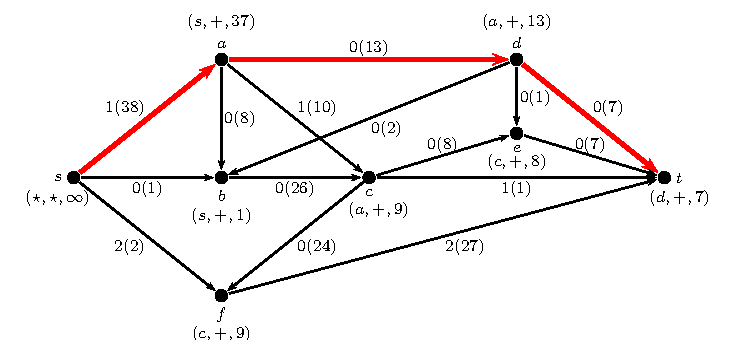
\includegraphics{fig25.pdf}
   \caption{$w(f_2) = 3$}
   \label{abb:9:4}
  \end{figure}
\end{center}
\end{frame}

\begin{frame}
 \frametitle{Weiterer Verlauf}
 \begin{center}
  \begin{figure}
   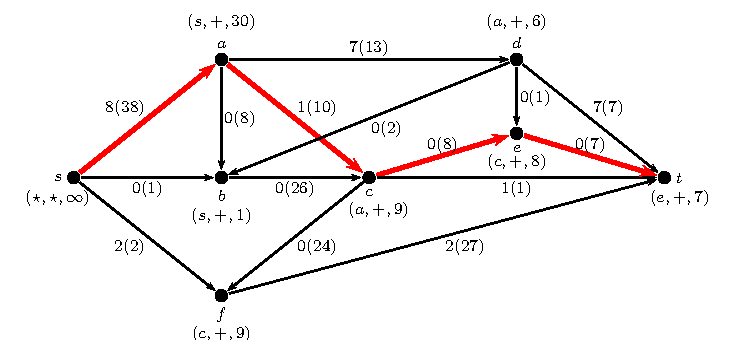
\includegraphics{fig26.pdf}
   \caption{$w(f_3) = 10$}
   \label{abb:9:5}
  \end{figure}
\end{center}
\end{frame}

\begin{frame}
 \frametitle{Weiterer Verlauf}
 \begin{center}
  \begin{figure}
   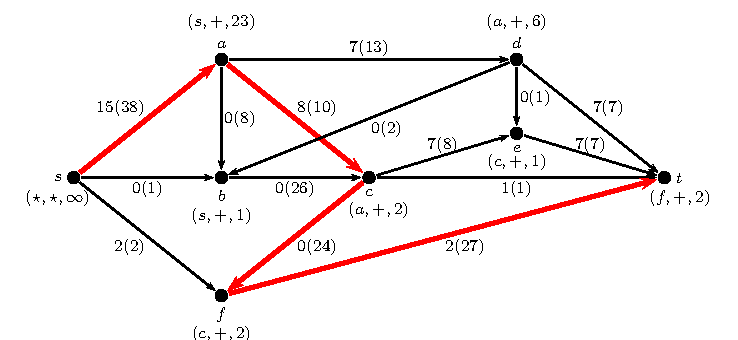
\includegraphics{fig27.pdf}
   \caption{$w(f_4) = 17$}
   \label{abb:9:6}
  \end{figure}
\end{center}
\end{frame}

\begin{frame}
 \frametitle{Weiterer Verlauf}
 \begin{center}
  \begin{figure}
   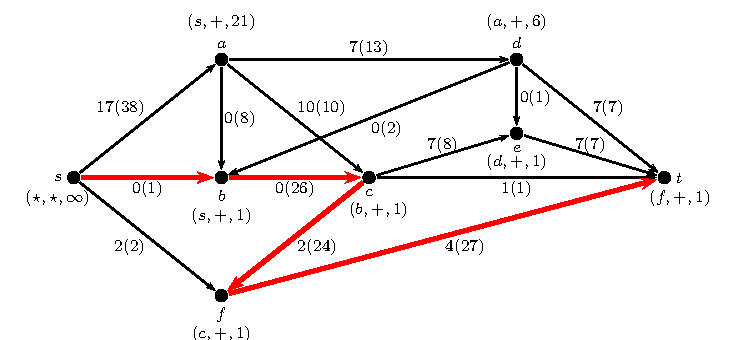
\includegraphics{fig28.pdf}
   \caption{$w(f_5) = 19$}
   \label{abb:9:7}
  \end{figure}
\end{center}
\end{frame}

\begin{frame}
 \frametitle{Weiterer Verlauf}
 \begin{center}
  \begin{figure}
   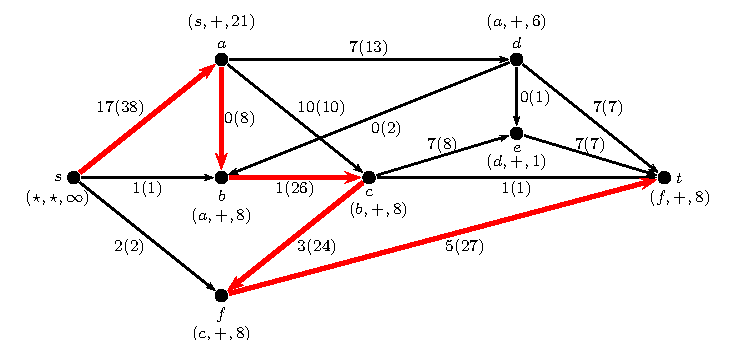
\includegraphics{fig29.pdf}
   \caption{$w(f_6) = 20$}
   \label{abb:9:8}
  \end{figure}
\end{center}
\end{frame}

\begin{frame}
 \frametitle{Weiterer Verlauf}
 \begin{center}
  \begin{figure}
   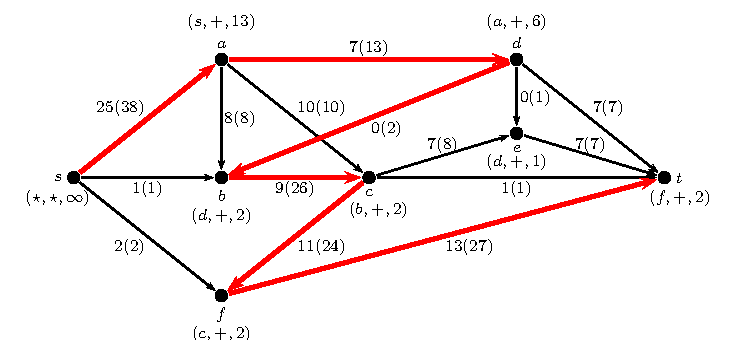
\includegraphics{fig30.pdf}
   \caption{$w(f_7) = 28$}
   \label{abb:9:9}
  \end{figure}
\end{center}
\end{frame}

\begin{frame}
 \frametitle{Weiterer Verlauf}
 \begin{center}
  \begin{figure}
   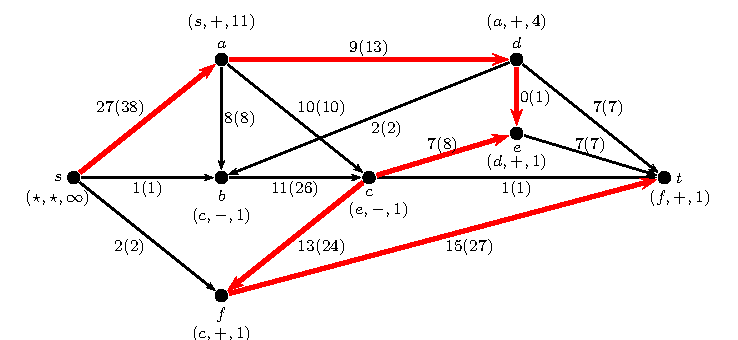
\includegraphics{fig31.pdf}
   \caption{$w(f_8) = 30$}
   \label{abb:9:10}
  \end{figure}
\end{center}
\end{frame}

\begin{frame}
 \frametitle{Weiterer Verlauf}
 \begin{center}
  \begin{figure}
   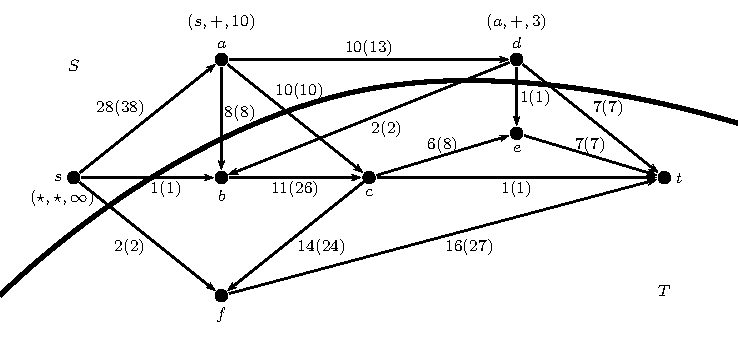
\includegraphics{fig32.pdf}
   \caption{$w(f_9) = 31 = c(S,T)$}
   \label{abb:9:11}
  \end{figure}
\end{center}
\end{frame}

\begin{frame}
\frametitle{Kleine Übung für die Weihnachtsferien}
\textbf{Zur Übung}:
\begin{enumerate}[a)]
\item Denken Sie sich in Abbildung \ref{abb:9:3} die Markierungen weg. Machen Sie sich Schritt für Schritt den Markierungsprozess klar, wobei Sie die Regel ($*$) beachten. Geben Sie auch immer den jeweils aktuellen Zustand von $Q$ an.
\item Wie kommt in Abbildung \ref{abb:9:3} der flussvergrößernde Pfad $s,a,c,t$ zustande? Wie kommt der in Abbildung \ref{abb:9:4} angegebene Fluss zustande?
\item Führen Sie die Überlegungen aus a) und b) ebenso für Abbildung \ref{abb:9:10} (anstelle von \ref{abb:9:3}) durch!
\item Führen Sie Entsprechendes auch für Abbildung \ref{abb:9:11} durch!
\end{enumerate}
\end{frame}

\begin{frame}
 \frametitle{Erreichbarkeit}
 Vor allem durch das vorangegangene, etwas umfangreichere Beispiel sollte klar geworden sein, dass es beim Algorithmus von Edmonds und Karp ganz wesentlich um \structure{Erreichbarkeit} von Knoten durch zunehmende Pfade geht. \\ \vspace*{0.2cm}

Wir führen die folgenden \textbf{Sprechweisen} ein: Anstatt zu sagen {\glqq}es gibt einen zunehmenden Pfad nach $w${\grqq} benutzen wir zukünftig auch Sprechweisen wie \\ \vspace*{0.2cm} 
\begin{itemize}
\item {\glqq}$w$ ist durch einen zunehmenden Pfad erreichbar{\grqq}, 
\item {\glqq}$w$ wurde durch einen zunehmenden Pfad erreicht{\grqq}.
\end{itemize}
\end{frame}

\begin{frame}
 \frametitle{Bedeutung der Knotenmarkierungen}
 Der Zusammenhang zwischen zunehmenden Pfaden und Knotenmarkierungen soll kurz angesprochen werden. Hierzu betrachten wir die Markierung
\[
(c,+,9)
\]
des Knotens $f$ in Abbildung \ref{abb:9:5}. Dass der Knoten $f$ markiert wurde bedeutet, dass $f$ im Laufe des Markierungsprozesses durch einen zunehmenden Pfad erreicht wurde; wir wollen diesen zunehmenden Pfad $P_f$ nennen. \\ \vspace*{0.2cm}

Der \alert{erste Eintrag} in der Markierung $(c,+,9)$ zeigt an, dass $c$ der Vorgänger von $f$ auf $P_f$ ist. \\ \vspace*{0.2cm}

Der \alert{zweite Eintrag} bedeutet, dass $f$ auf einer Vorwärtskante erreicht wurde; mit anderen Worten: Die Vorwärtskante $(c,f)$ ist die letzte Kante auf $P_f$. (Wäre $f$ auf einer Rückwärtskante erreicht worden, so wäre der zweite Eintrag ein Minuszeichen gewesen.)
\end{frame}

\begin{frame}
 \frametitle{Bedeutung der Knotenmarkierungen}
 Der \alert{dritte Eintrag} gibt die Größe des \structure{Flaschenhalses} von $P_f$ an. Um zu erkennen, was damit gemeint ist, bestimmen wir den gesamten Pfad $P_f$: \vspace*{0.2cm}
 \begin{itemize}
 \item Der Knoten $c$ ist mit $(a,+,9)$ markiert, d.h.,  $a$ ist der Vorgänger von $c$ auf $P_f$; 
 \item der Knoten $a$ ist mit $(s,+,30)$ markiert, d.h., $s$ ist der Vorgänger von $a$ auf $P_f$.
 \end{itemize}
 
 \vspace*{0.2cm}
 Somit lautet der Pfad $P_f$ wie folgt:
 \[
 P_f:\ s,\ a,\ c,\ f.
 \]
\end{frame}

\begin{frame}
 \frametitle{Der Flaschenhals}
 Der Pfad $P_f$ durchläuft seine drei Kanten $e_1=(s,a)$, $e_2=(a,c)$ und $e_3=(c,f)$ in Vorwärtsrichtung, weshalb für alle drei Kanten die Differenz zwischen der Kapazität und dem aktuellen Fluss betrachtet wird: \vspace*{0.2cm}
 \begin{itemize}
 \item Im Fall von $e_1$ beträgt diese Differenz $38-8=30$,
 \item im Fall von $e_2$ erhält man $10-1=9$, 
 \item und für $e_3$ ergibt sich $24-0=24$.
 \end{itemize}
 
 \vspace*{0.2cm}
 \alert{Der kleinste Wert ist also $9$} -- und genau dies liest man an der Markierung $(c,+,9)$ in der dritten Stelle ab. Woher der Ausdruck \structure{{\glqq}Größe des Flaschenhalses{\grqq}} kommt und weshalb man $e_2$ als \structure{{\glqq}Flaschenhalskante{\grqq}} bezeichnet, sollte aufgrund der vorangegangenen Ausführungen klar sein.
\end{frame}

\begin{frame}
 \frametitle{Komplexität des Algorithmus von Edmonds und Karp}
 Die Komplexität des Algorithmus von Edmonds und Karp ist \alert{$O(nm^2)$} für $n=|V|$ und $m=|E|$. \\ \vspace*{0.2cm}
 
 \alert{Wir skizzieren, weshalb dies so ist:} Das Auffinden eines zunehmenden Pfades (bzw. im letzten Schritt die vergebliche Suche nach einem solchen) ist in $O(m)$ Schritten durchführbar, da jede Kante höchstens zweimal untersucht wird; und beim anschließenden Ändern des Flusses ist jede Kante höchstens einmal involviert. \\ \vspace*{0.2cm}
 
 Da es nach dem Satz von Edmonds und Karp nur $O(nm)$ Flussvergrößerungen gibt, folgt insgesamt die Komplexitätsschranke $O(nm^2)$.
\end{frame}

\begin{frame}
 \frametitle{Bemerkung zur Darstellung von $G$}
 Wie bisher bezeichne $G=(V,E)$ den gerichteten Graphen des Netzwerks $N$. Wir schließen diesen Abschnitt mit einer Bemerkung zur \alert{Darstellung von $G$}. Es bietet sich als Standardlösung an, $G$ durch \structure{Adjazenzlisten} darzustellen. Dabei ist es zweckmäßig, zu jedem Knoten $v$ \alert{zwei} Adjazenzlisten zur Verfügung zu haben: \\ \vspace*{0.2cm}
\begin{itemize}
\item Die erste Liste enthält sämtliche Knoten $y$, für die $(v,y) \in E$ gilt.
\item Die zweite Liste enthält sämtliche Knoten $x$, für die $(x,v) \in E$ gilt.
\end{itemize}
\vspace*{0.2cm}

Beide Listen kommen zum Einsatz, wenn im Labelling-Algorithmus die Repeat-Schleife durchlaufen wird: Die erste Liste wird durchlaufen, wenn die Zeilen (6)--(11) abgearbeitet werden; die zweite Liste wird anschließend verwendet, wenn es um die Zeilen (12)--(17) geht.  \\ \vspace*{0.2cm}

Sind die Knoten mit Buchstaben bezeichnet und sind beide Listen alphabetisch geordnet, so entspricht dies gerade der Regel ($*$) auf Folie \pageref{page:9:8}.
\end{frame}

\begin{frame}
 \frametitle{Ähnlichkeiten zwischen Labelling- und Simplexalgorithmus}
 Man kann viele \alert{Ähnlichkeiten} zwischen dem Labelling-Algorithmus und dem Simplexalgorithmus beobachten, beispielsweise diese: Am Schluss, wenn keine Verbesserung mehr möglich ist, erhält man in beiden Fällen eine \alert{{\glqq}Zugabe{\grqq}}; genauer gilt: \\ \vspace*{0.2cm}
 \begin{itemize}
  \item Beim Simplexalgorithmus erhält man zusätzlich eine optimale Lösung   
      des dualen Problems;
  \item Beim Labelling-Algorithmus erhält man neben einem maximalen Fluss 
     auch einen minimalen Schnitt.
 \end{itemize}
 \vspace*{0.2cm}
 
Auf diese Ähnlichkeit werden wir später noch eingehen.
\end{frame}

\end{document}
